\documentclass{standalone}
\usepackage{tikz}
\usepackage{tikz-qtree}
\usepackage[makeroom]{cancel}
\usetikzlibrary{fit}


\begin{document} 
	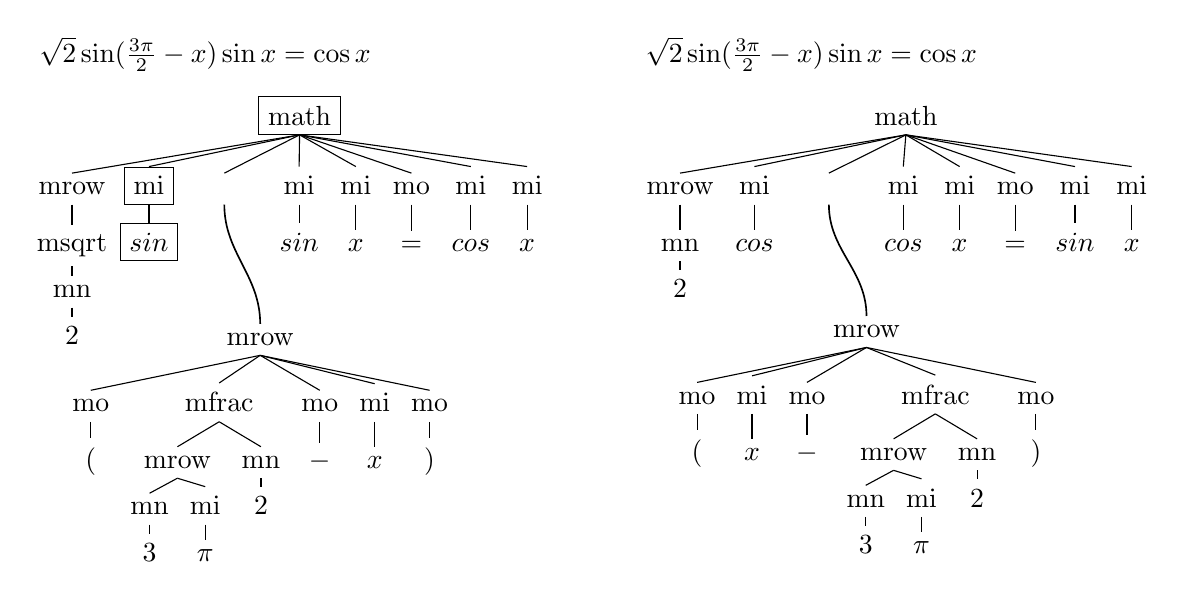
\begin{tikzpicture}[sibling distance=1.2pt]
	\tikzset{level 1/.style={level distance=2.1\baselineskip}}
	\tikzset{level 2/.style={level distance=1.7\baselineskip}}
	\tikzset{level 3+/.style={level distance=1.4\baselineskip}}

	    \node (x) at (-1.2,0.9) {$\sqrt{2}\sin (\frac{3\pi}{2} - x)\sin x = \cos x$};
	    \Tree [.\node[draw]{math};
	    		[.mrow 
	    			[.msqrt 
	    				[.mn
	    					[.$2$ ]
	    				]
	    			]
	    		]
	    		[.\node[draw]{mi}; \node[draw]{$sin$}; ]
	    		[.\node(m2){\phantom{mrow}}; ]
	    		[.mi $sin$ ]
	    		[.mi $x$ ]
	    		[.mo $=$ ]
	    		[.mi $cos$ ]
	    		[.mi $x$ ]
	          ]
	    

		\begin{scope}[xshift=-.5cm, yshift=-2.8cm]
		\tikzset{level 1/.style={level distance=2.0\baselineskip}}
		\tikzset{level 2+/.style={level distance=1.55\baselineskip}}
		\tikzset{level 1+/.style={sibling distance=0.08\baselineskip}}
		\Tree [.\node(m1){mrow}; 
	    			[.mo $($ ]
	    			[.mfrac 
	    				[.mrow 
	    					[.mn $3$ ]
	    					[.mi $\pi$ ]
	    				]
	    				[.mn $2$ ]
	    			]
	    			[.mo $-$ ]
	    			[.mi $x$ ]
	    			[.mo $)$ ]
	    	  ]
		\draw[semithick,-] (m1) to [out=90, in=270] (m2);
		\end{scope}


		\begin{scope}[xshift=7.7cm]
			\tikzset{level 1/.style={level distance=2.1\baselineskip}}
			\tikzset{level 2+/.style={level distance=1.7\baselineskip}}
		    \node (x) at (-1.2,0.9) {$\sqrt{2}\sin (\frac{3\pi}{2} - x)\sin x = \cos x$};
		    \Tree [.math
		    		[.mrow 
		    			[.mn
		    				[.$2$ ]
		    			]
		    		]
		    		[.mi $cos$ ]
		    		[.\node(m2){\phantom{mrow}}; ]
		    		[.mi $cos$ ]
		    		[.mi $x$ ]
		    		[.mo $=$ ]
		    		[.mi $sin$ ]
		    		[.mi $x$ ]
		          ]
		\end{scope}

		\begin{scope}[xshift=7.2cm, yshift=-2.7cm]
			\tikzset{level 1/.style={level distance=2.0\baselineskip}}
			\tikzset{level 2+/.style={level distance=1.55\baselineskip}}
			\tikzset{level 1+/.style={sibling distance=0.08\baselineskip}}
			\Tree [.\node(m1){mrow}; 
		    			[.mo $($ ]
		    			[.mi $x$ ]
		    			[.mo $-$ ]
		    			[.mfrac 
		    				[.mrow 
		    					[.mn $3$ ]
		    					[.mi $\pi$ ]
		    				]
		    				[.mn $2$ ]
		    			]
		    			[.mo $)$ ]
		    	  ]
			\draw[semithick,-] (m1) to [out=90, in=270] (m2);
		\end{scope}



	\end{tikzpicture}
\end{document} 